\documentclass[conference]{IEEEtran}

\usepackage{cite}
\usepackage{amsmath,amssymb,amsfonts}
\DeclareMathOperator{\Tr}{Tr}

\usepackage{bm}
\usepackage{algorithmic}
\usepackage{graphicx}
\usepackage{textcomp}
\usepackage{xcolor}
\def\BibTeX{{\rm B\kern-.05em{\sc i\kern-.025em b}\kern-.08em
    T\kern-.1667em\lower.7ex\hbox{E}\kern-.125emX}}
\begin{document}

\title{Statistical Properties of Geodesic Distances between Samples and Elementary Backscatterers in PolSAR Imagery}

\author{\IEEEauthorblockN{Danilo Fernandes, 
Alejandro C.\ Frery,~\IEEEmembership{Senior Member,~IEEE}}
\IEEEauthorblockA{Laborat\'orio de Computa\c c\~ao Cient\'ifica e An\'alise Num\'erica\\
Universidade Federal de Alagoas\\
Macei\'o, Brazil\\
Email: dfc@laccan.ufal.br, acfrery@laccan.ufal.br
%acfrery@laccan.ufal.br
%\and  
%\IEEEauthorblockN{2\textsuperscript{nd} Danilo Fernandes}
%\IEEEauthorblockA{\textit{Laborat\'orio de Computa\c c\~ao Cient\'ifica e An\'alise Num\'erica} \\
%\textit{Universidade Federal de Alagoas}\\
%Macei\'o, Brazil \\
%dfc@laccan.ufal.br}
}}

\maketitle

\begin{abstract}
PolSAR data are usually represented by complex scattering or covariance matrices.
Another representation is by Kennaugh matrices, which are real and preserve the backscatter information.
This approach allows measuring distances and, consequently, the dissimilarity between PolSAR data and known backscatters.
In this report, we analyze the statistical properties of this dissimilarity measure between PolSAR data samples and elementary backscatters using a Geodesic Distance.
\end{abstract}

% Note that keywords are not normally used for peerreview papers.
\begin{IEEEkeywords}
PolSAR, Kennaugh matrix, Geodesic Distance.
\end{IEEEkeywords}

\section{Introduction}
\IEEEPARstart{I}{n} Polarimetric SAR, a radar target is characterized by a scattering matrix $\bm S$ that describes the dependence of its scattering properties on the polarization. 
It is defined as
\[\bm{S} = 
\begin{bmatrix}
S_{\text{HH}} & S_{\text{HV}}\\
S_{\text{VH}} & S_{\text{VV}}\\
\end{bmatrix}
,\]
where $\text{H}$ and $\text{V}$ denote, respectively, horizontal and vertical polarization.

This information can be projected and then visualized using the Pauli vector representation:
$\bm{k} = 2^{-1/2} 
\begin{bmatrix}
S_{\text{HH}} + S_{\text{VV}} &S_{\text{HH}} - S_{\text{VV}} &2S_{\text{HV}}
\end{bmatrix}^T
$, 
where $T$ denotes transposition. 
Another important matrix in PolSAR theory is the coherency $\bm{T}$ obtained by:
$$
\bm{T} = \frac{1}{L} \sum_{\ell=1}^{L}\textbf{k}_\ell \textbf{k}_\ell^{*T},
$$
where $*$ denotes the complex conjugate, and $L$ is the number of looks.

The Kennaugh matrix $\bm{K}$ can be obtained from the coherency matrix $\bm{T}$:
\[
\begin{bmatrix}
\frac{ T_{11} + T_{22} + T_{33} }{2} & \Re(T_{12}) & \Re(T_{13}) & \Im(T_{23})\\
\Re(T_{12}) & \frac{T_{11} + T_{22} - T_{33}}{2} & \Re(T_{23}) & \Im(T_{13})\\
\Re(T_{13}) & \Re(T_{23}) & \frac{ T_{11} - T_{22} + T_{33} }{2} & -\Im(T_{12})\\
\Im(T_{23}) & \Im(T_{13}) & -\Im(T_{12}) & \frac{ -T_{11} + T_{22} + T_{33} }{2}\\
\end{bmatrix}
.\]

The Geodesic Distance between two Kennaugh matrices $\bm K_1$ and $\bm K_2$ is~\cite{ClassificationPolSARGeodesic}: 
\begin{displaymath}
\text{GD}(\bm K_1, \bm K_2) = \frac{2}{\pi} \cos^{-1} \left(\frac{\Tr(\bm K_1^T \bm K_2)}{\sqrt{\Tr(\bm K_1^T \bm K_1)} \sqrt{\Tr(\bm K_2^T \bm K_2})} \right),
\end{displaymath}
where $\Tr$ denotes the trace.
It ranges between $[0,1]$.
%This leads to defining a measure of similarity between PolSAR data: $f(\bm K_1, \bm K_2) = 1 - \text{GD}(\bm K_1, \bm K_2)$. 
This measure of dissimilarity has been used to 
classify images~\cite{ClassificationPolSARGeodesic},
in the proposal of a new generalized volume scattering model~\cite{AGeneralizedVolumeScatteringModelBasedVegetationIndexfromPolarimetricSARData2019},
and for the analysis of built-up areas~\cite{NovelTechniquesforBuiltupAreaExtractionfromPolarimetricSARImages2019}.

In this work, we are interested in the dissimilarity between samples and elementary backscatterers:
trihedral, dihedral, random volume, narrow dihedral, cylinder, dipole, left helix, right helix, $+1/4$-wave and $-1/4$-wave, whose Kennaugh matrices are, respectively:
\[K_a =
\begin{bmatrix}
1 & 0 & 0 & 0\\
0 & 1 & 0 & 0\\
0 & 0 & 1 & 0\\
0 & 0 & 0 & -1\\
\end{bmatrix},
K_b =
\begin{bmatrix}
1 & 0 & 0 & 0\\
0 & 1 & 0 & 0\\
0 & 0 & -1 & 0\\
0 & 0 & 0 & 1\\
\end{bmatrix},
\]
\[K_{rv} =
\begin{bmatrix}
1 & 0 & 0 & 0\\
0 & 1/2 & 0 & 0\\
0 & 0 & 1/2 & 0\\
0 & 0 & 0 & 0\\
\end{bmatrix},
K_{nd} =
\begin{bmatrix}
5/8 & 3/8 & 0 & 0\\
3/8 & 5/8 & 0 & 0\\
0 & 0 & -1/2 & 0\\
0 & 0 & 0 & 1/2
\end{bmatrix},
\]
\[K_{c} =
\begin{bmatrix}
5/8 & 3/8 & 0 & 0\\
3/8 & 5/8 & 0 & 0\\
0 & 0 & 1/2 & 0\\
0 & 0 & 0 & -1/2\\
\end{bmatrix},
K_d=
\begin{bmatrix}
1 & -1 & 0 & 0\\
-1 & 1 & 0 & 0\\
0 & 0 & 0 & 0\\
0 & 0 & 0 & 0\\
\end{bmatrix},
\]
\[K_{lh}=
\begin{bmatrix}
1 & 0 & 0 & -1\\
0 & 0 & 0 & 0\\
0 & 0 & 0 & 0\\
-1 & 0 & 0 & 1\\
\end{bmatrix},
K_{rh}=
\begin{bmatrix}
1 & 0 & 0 & 1\\
0 & 0 & 0 & 0\\
0 & 0 & 0 & 0\\
1 & 0 & 0 & 1\\
\end{bmatrix}
,\]

\[K_{+1/4}=
\begin{bmatrix}
1 & 0 & 0 & 0\\
0 & 1 & 0 & 0\\
0 & 0 & 0 & 1\\
0 & 0 & 1 & 0\\
\end{bmatrix},
K_{-1/4}=
\begin{bmatrix}
1 & 0 & 0 & 0\\
0 & 1 & 0 & 0\\
0 & 0 & 0 & -1\\
0 & 0 & -1 & 0\\
\end{bmatrix}
.\]

In this report is presented histograms of similarities between aforementioned elementary backscatters and PolSAR data of forest and bare soil regions. 
The used data is from UAVSAR and corresponding to Sierra  del  Lacandon  National  Park,  Guatemala. 

\section{Histograms of similarities}

For the construction of the histograms, it was selected the PolSAR data with dimension of 50x50 pixels referent to a forest region and a bare soil region belong to Sierra  del  Lacandon  National  Park. This histograms are showed in the figures \ref{fig:wvn} to \ref{fig:tr}. Observe that the histograms referent to the same elementary backscatterer are different to forest and bare soil regions. In this way, the statistical behavior of the Geodesic Distance between PolSAR data and elementary backscatterers allows to characterize forest and bare soil regions.

%Code generator of these histograms is in Code folder in this repository
\begin{figure}[!ht]
    \vspace{.151\linewidth}
    \centering
    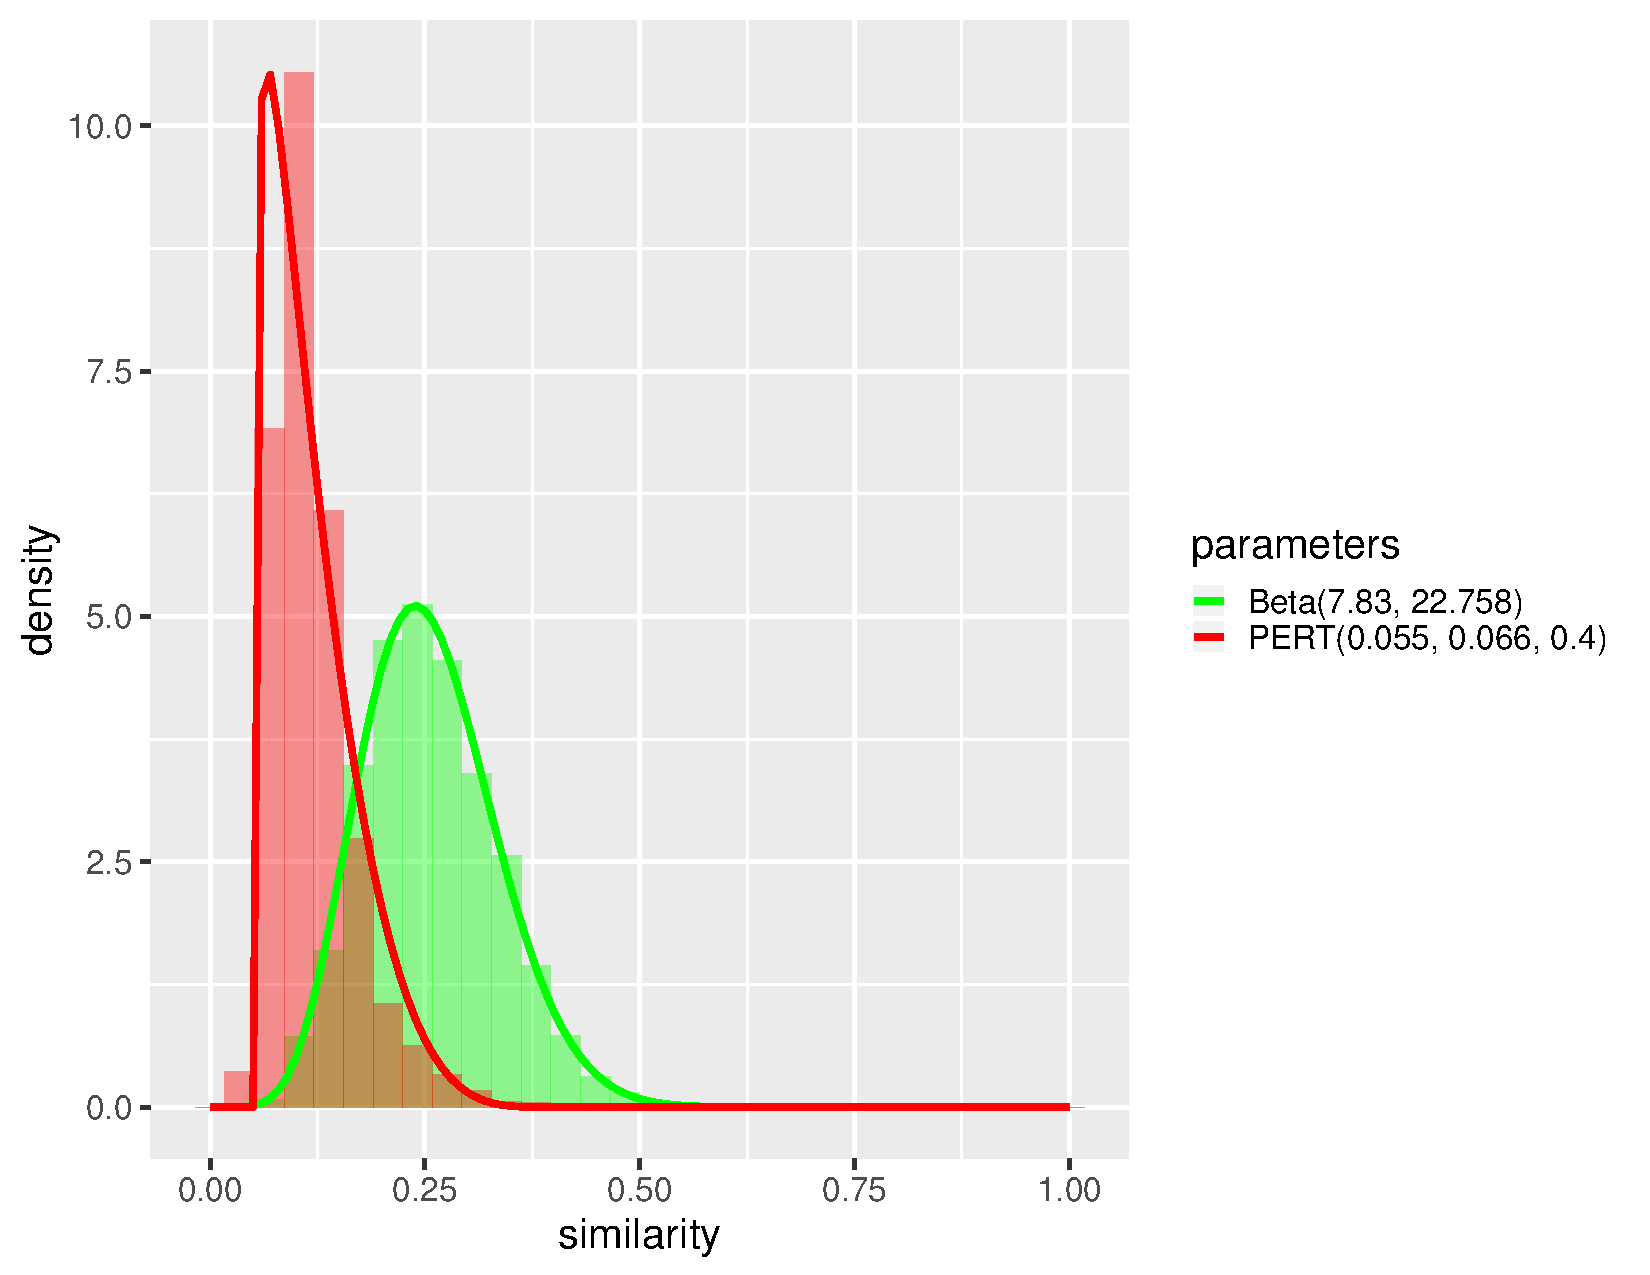
\includegraphics[width = .9\linewidth, height = .7\linewidth]{../../../Figures/paper_19_05/wvn.pdf}
    \caption{Similarity between $-1/4$-wave elementary backscatterer and PolSAR data from the forest region and bare soil region }
    \label{fig:wvn}
\end{figure}

\begin{figure}[!ht]
    \vspace{.15\linewidth}
    \centering
    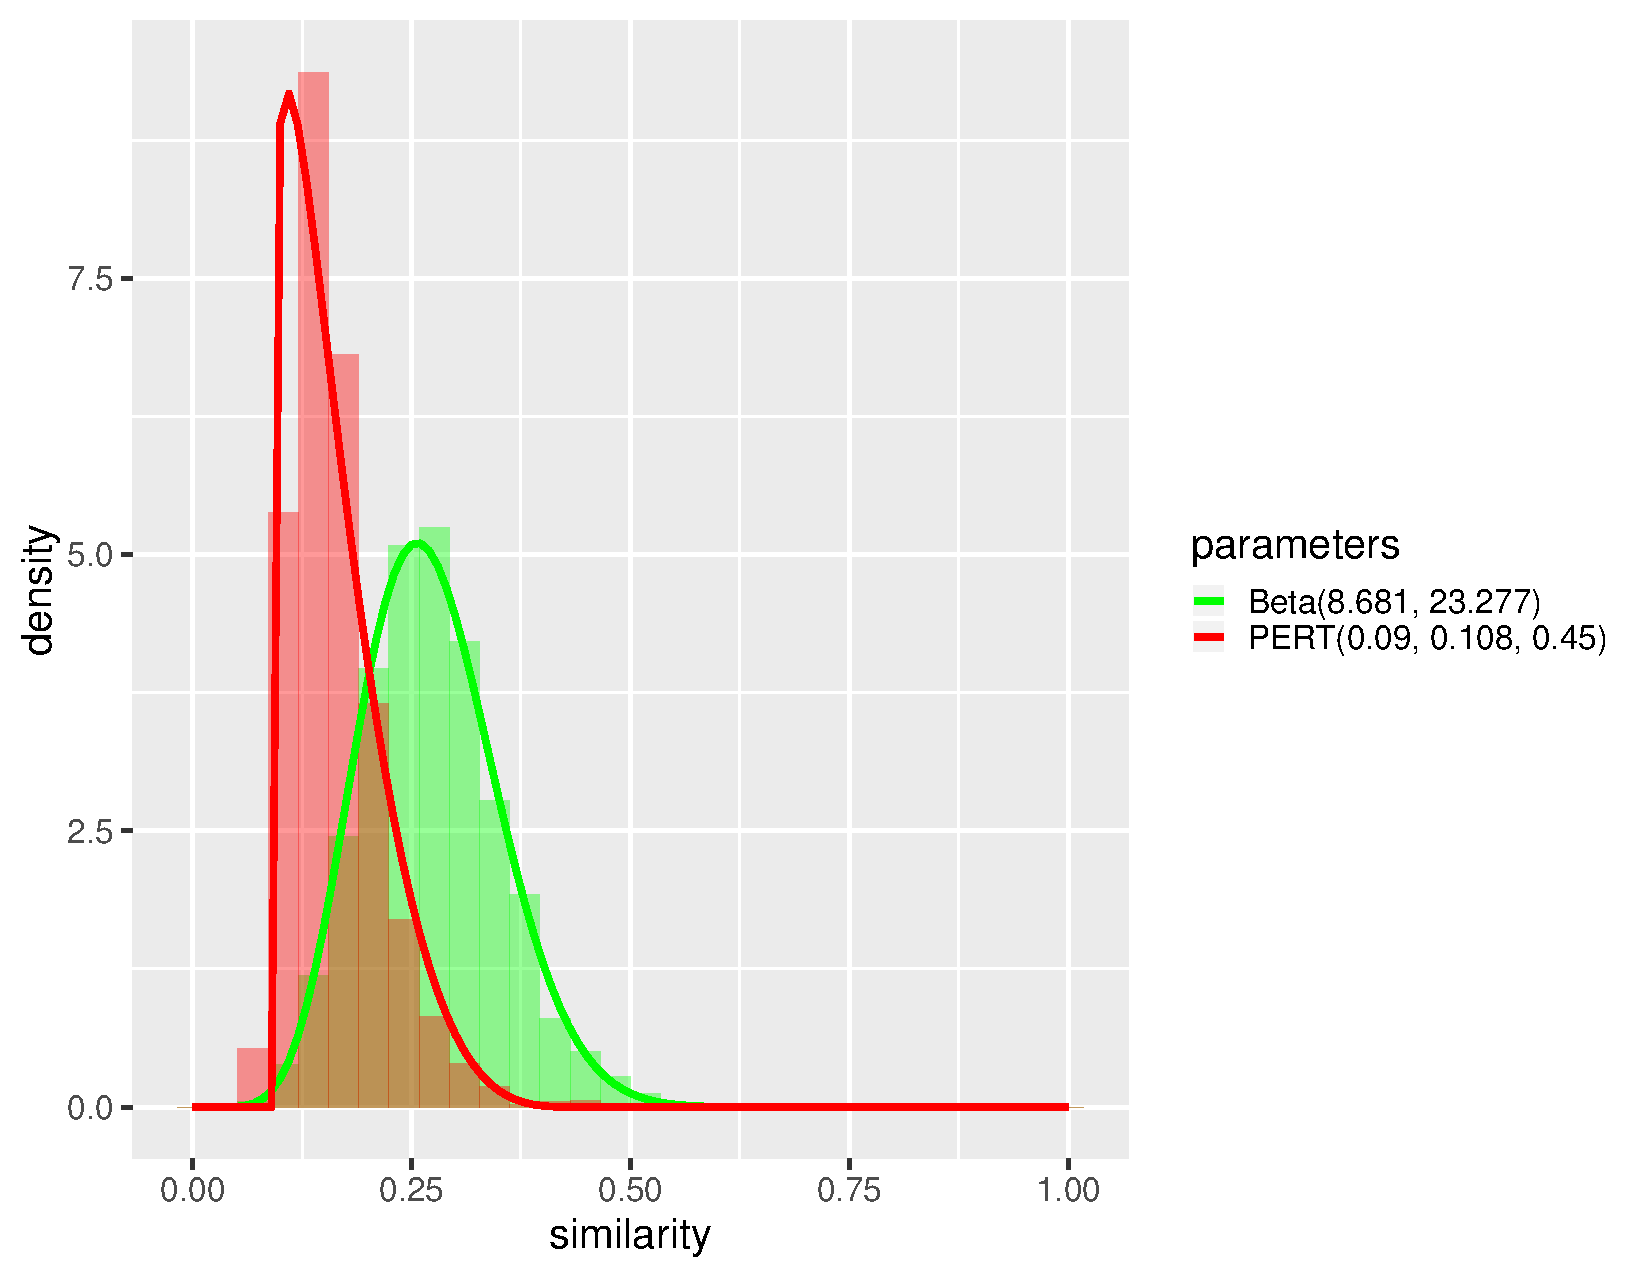
\includegraphics[width = .9\linewidth, height = .7\linewidth]{../../../Figures/paper_19_05/wvp.pdf}
    \caption{Similarity between $+1/4$-wave elementary backscatterer and PolSAR data from the forest region and bare soil region}
    \label{fig:wvp}
\end{figure}

\begin{figure}[!ht]
    \centering
    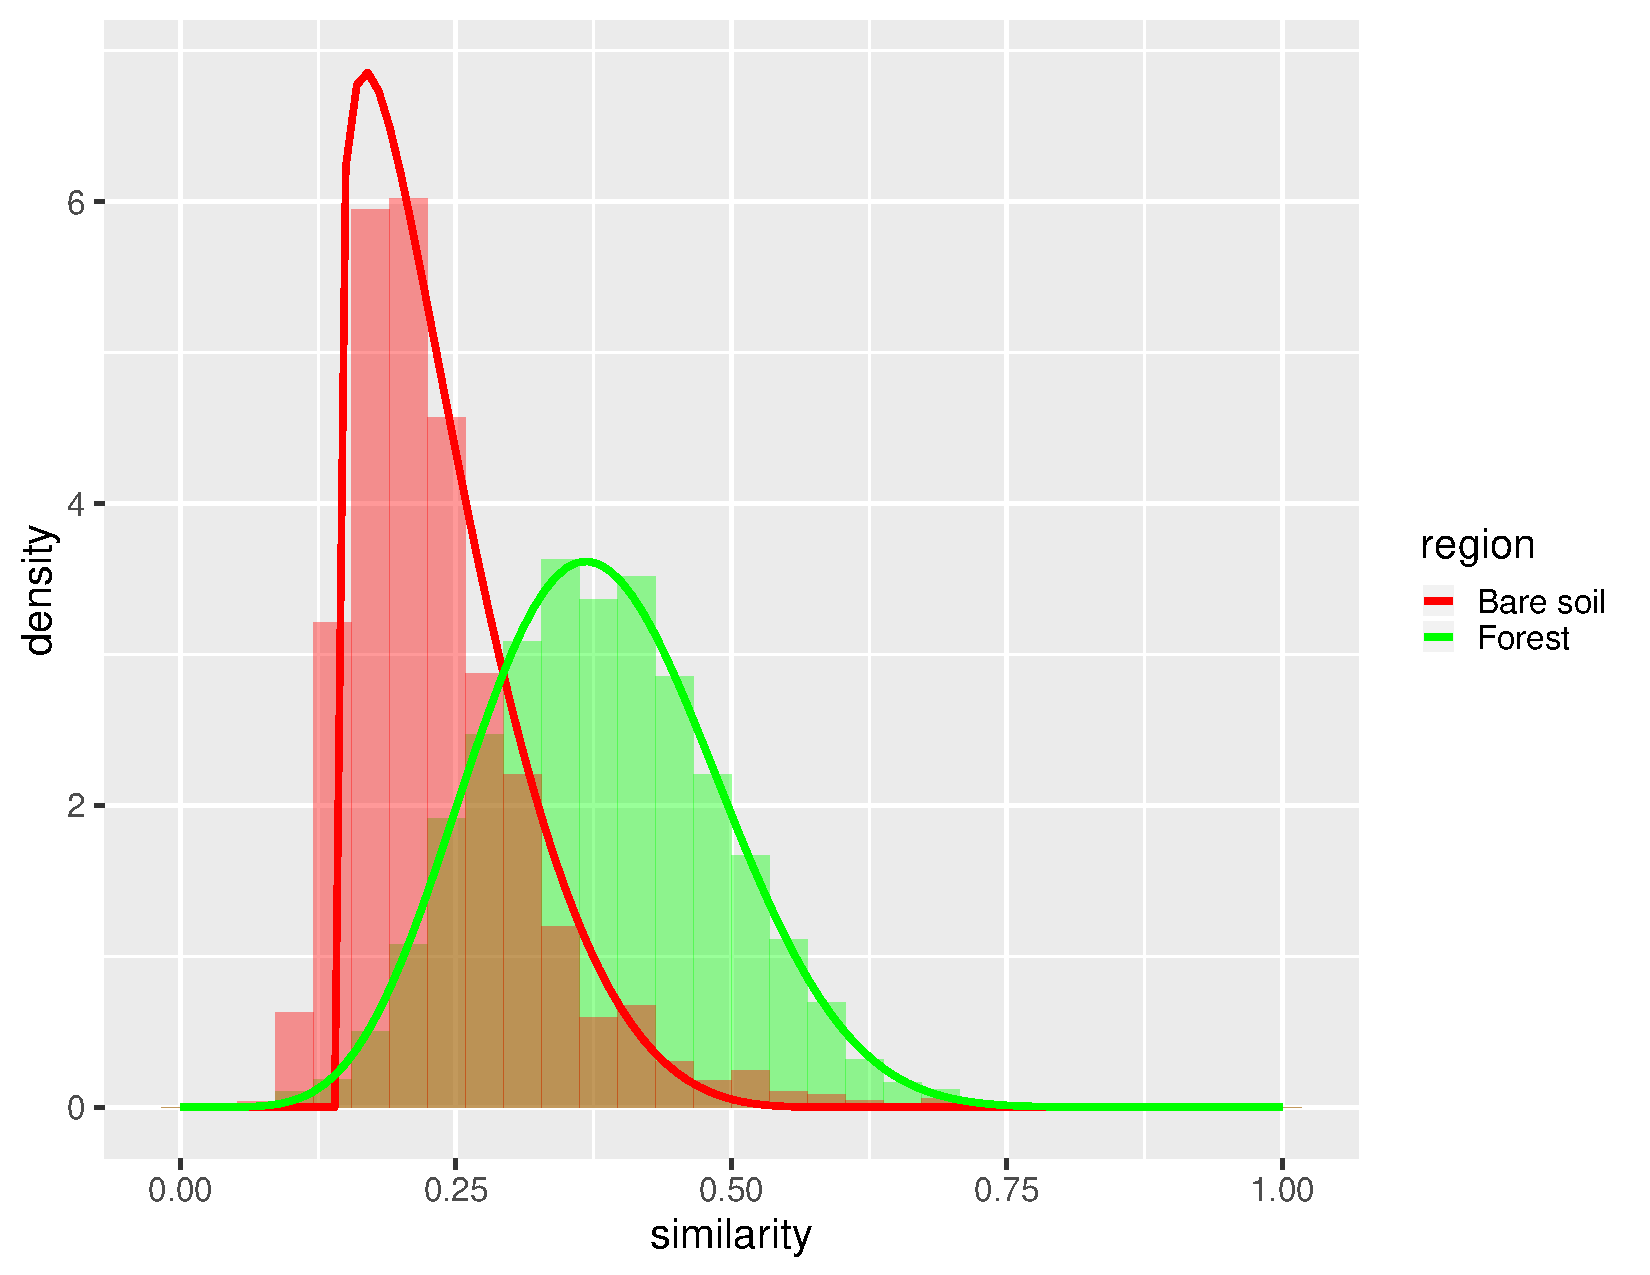
\includegraphics[width = .9\linewidth, height = .7\linewidth]{../../../Figures/paper_19_05/cy.pdf}
    \caption{Similarity between cylinder elementary backscatterer and PolSAR data from the forest region (in green) and bare soil region (in red)}
    \label{fig:cy}
\end{figure}

\begin{figure}[!ht]
    \centering
    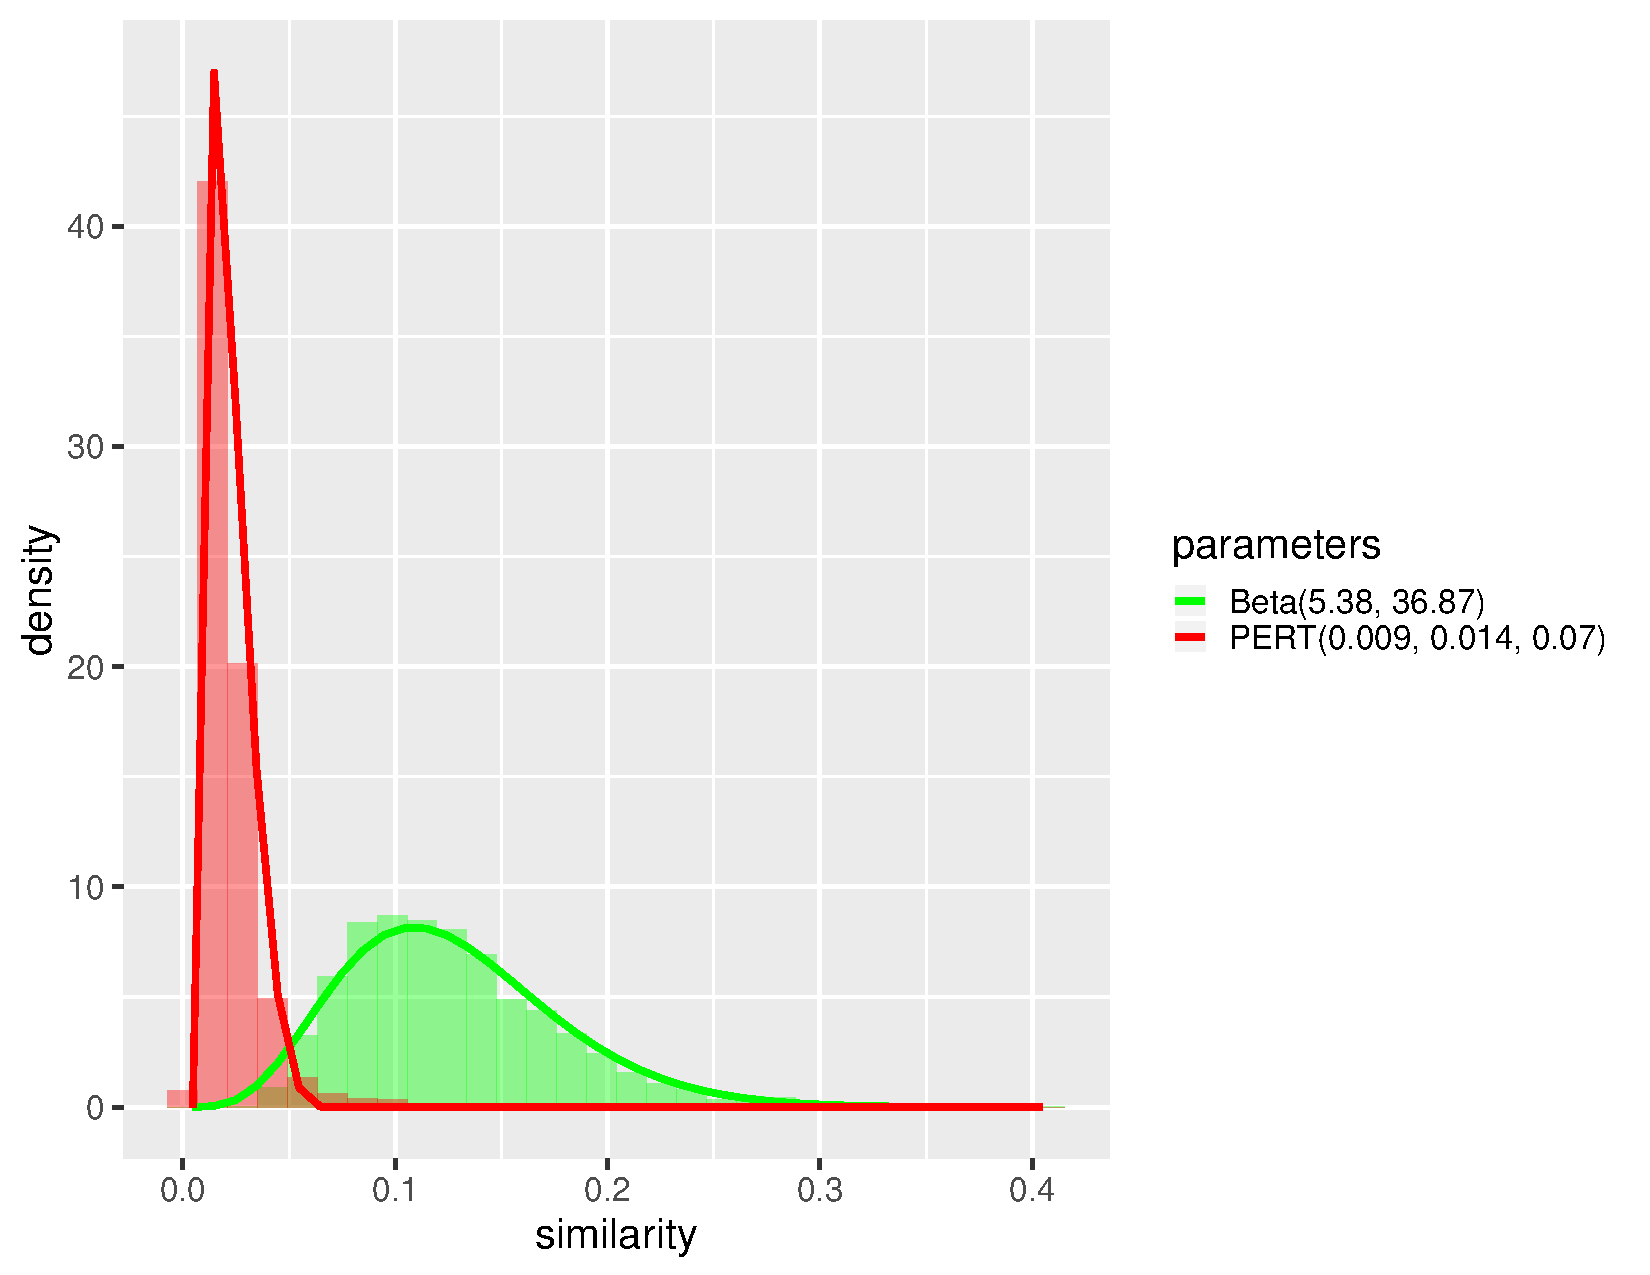
\includegraphics[width = .9\linewidth, height = .7\linewidth]{../../../Figures/paper_19_05/di.pdf}
    \caption{Similarity between dihedral elementary backscatterer and PolSAR data from the forest region (in green) and bare soil region (in red)}
    \label{fig:di}
\end{figure}

\begin{figure}[!ht]
    \centering
    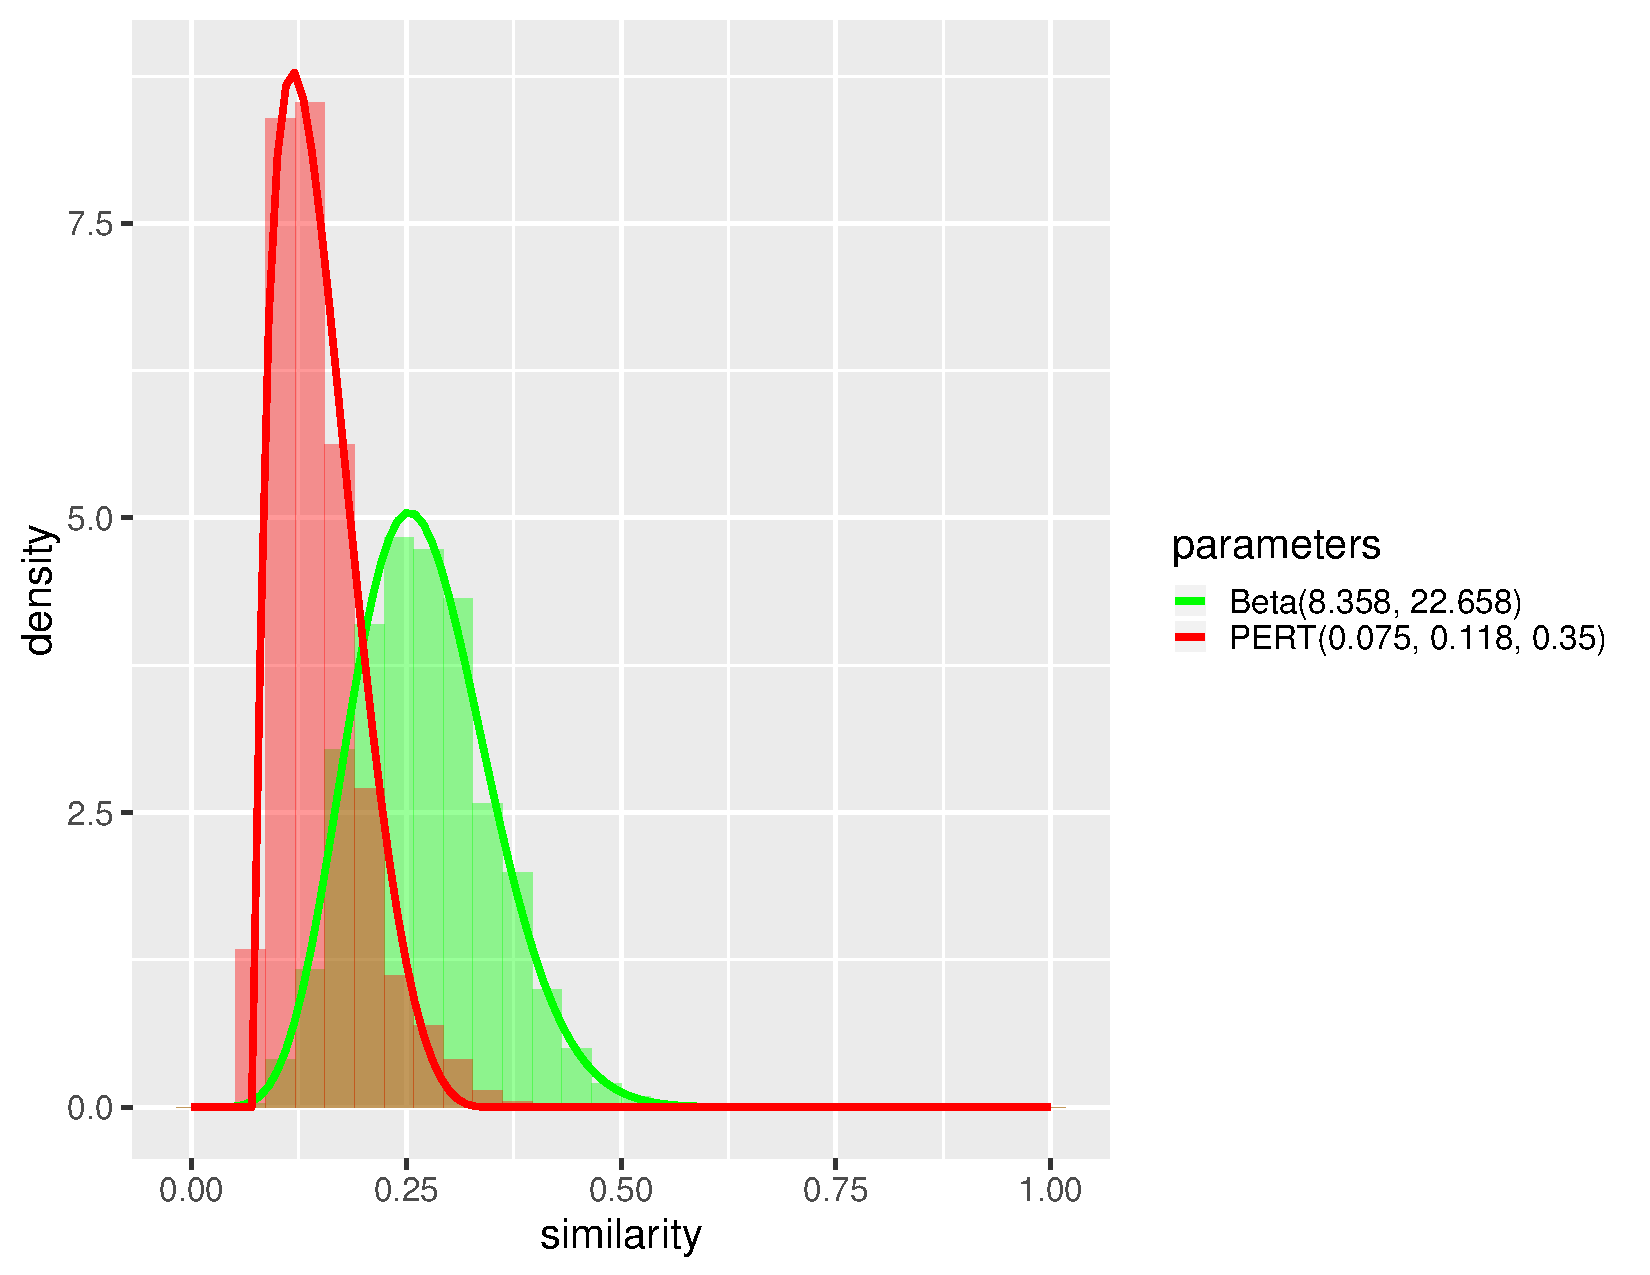
\includegraphics[width = .9\linewidth, height = .7\linewidth]{../../../Figures/paper_19_05/dip.pdf}
    \caption{Similarity between dipole elementary backscatterer and PolSAR data from the forest region (in green) and bare soil region (in red)}
    \label{fig:dip}
\end{figure}

\begin{figure}[!ht]
    \centering
    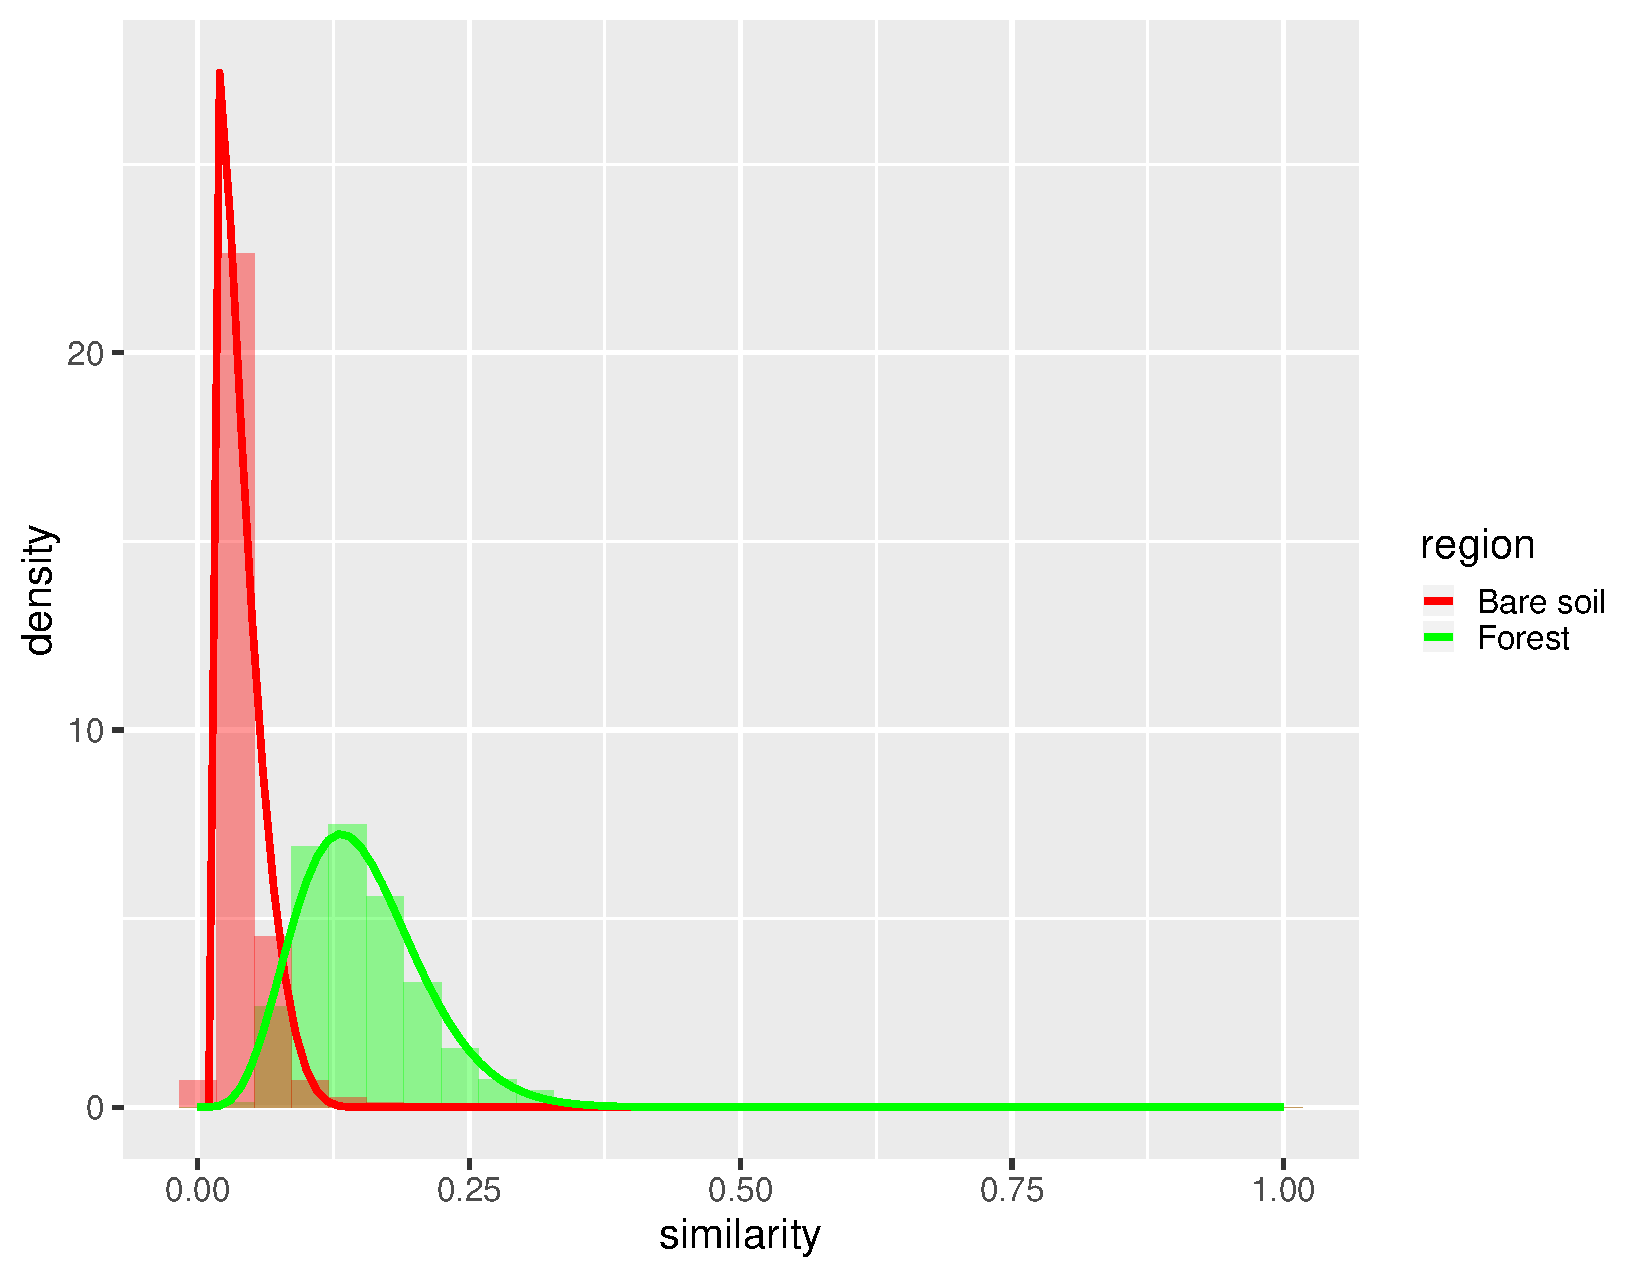
\includegraphics[width = .9\linewidth, height = .7\linewidth]{../../../Figures/paper_19_05/nd.pdf}
    \caption{Similarity between narrow dihedral elementary backscatterer and PolSAR data from the forest region (in green) and bare soil region (in red)}
    \label{fig:nd}
\end{figure}

\begin{figure}[!ht]
    \centering
    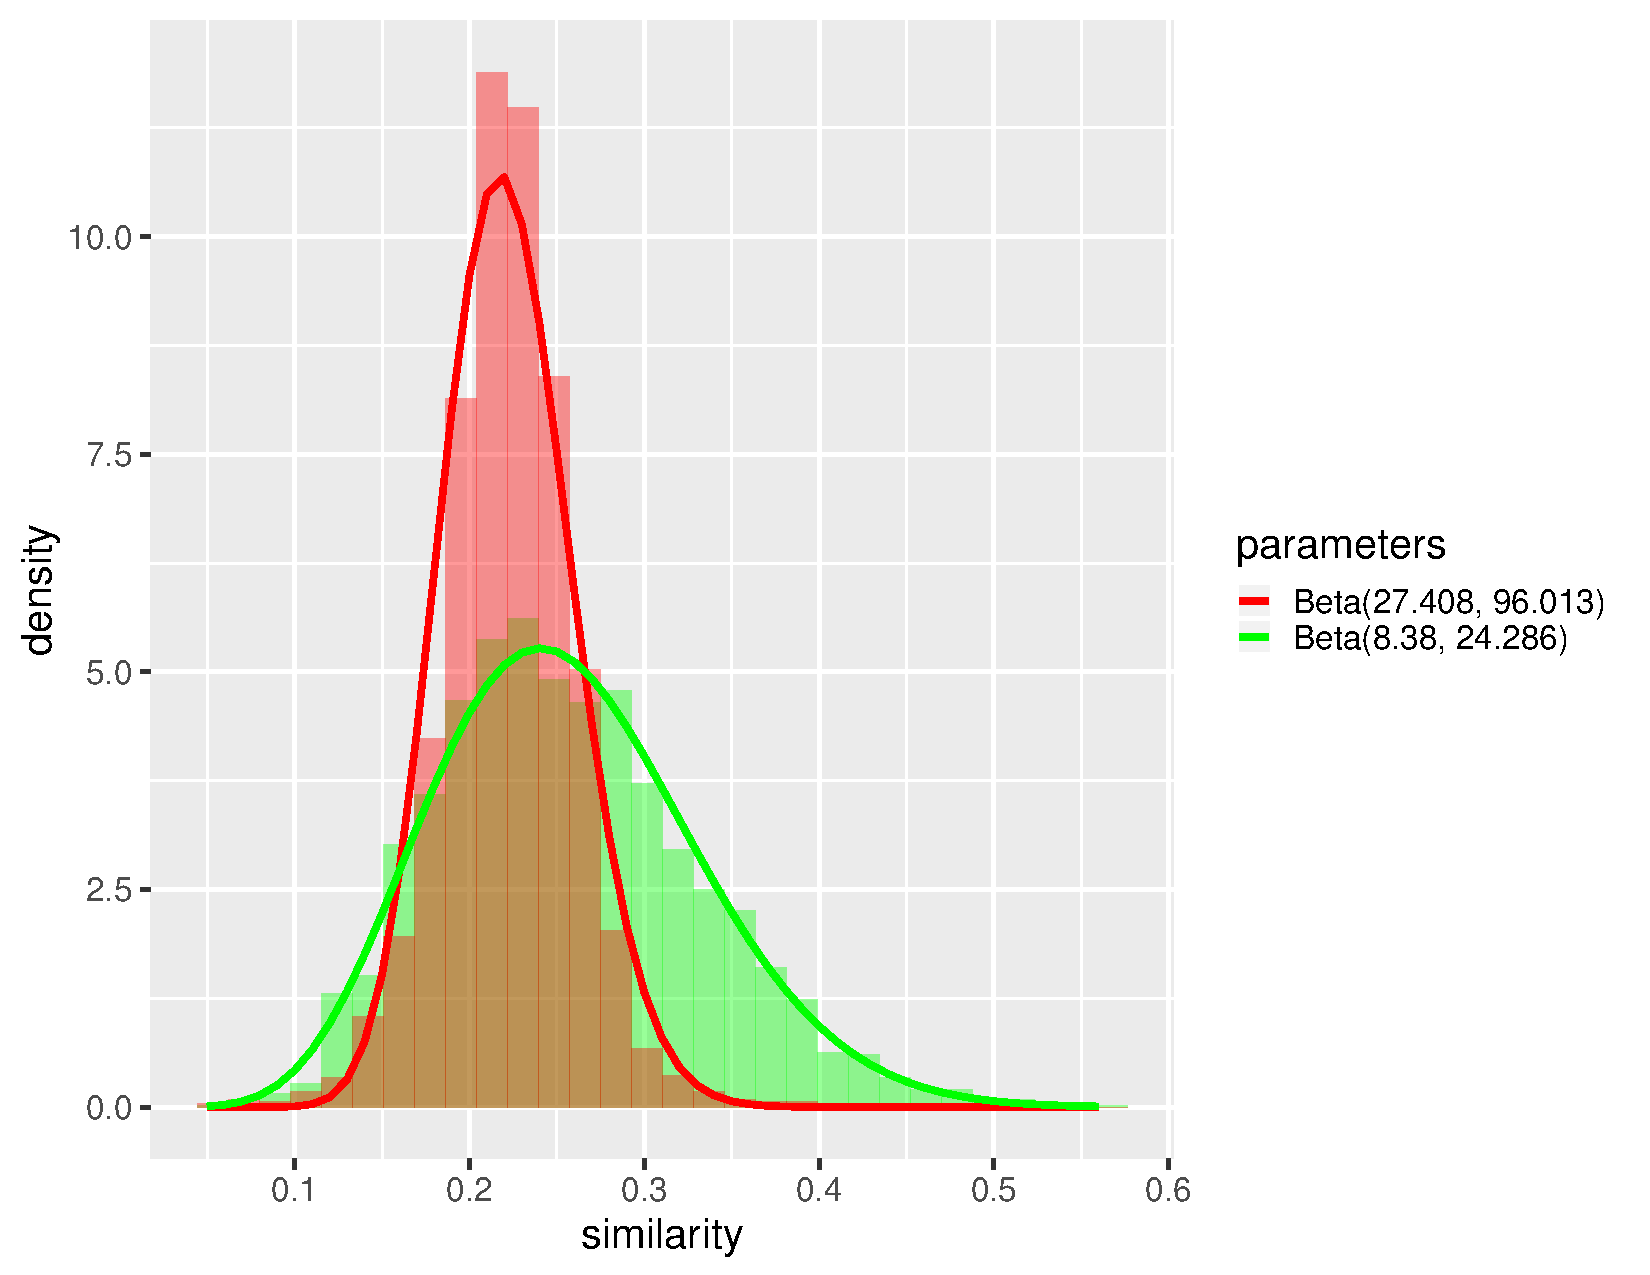
\includegraphics[width = .9\linewidth, height = .7\linewidth]{../../../Figures/paper_19_05/lh.pdf}
    \caption{Similarity between left helix elementary backscatterer and PolSAR data from the forest region (in green) and bare soil region (in red)}
    \label{fig:lh}
\end{figure}

\begin{figure}[!ht]
    \centering
    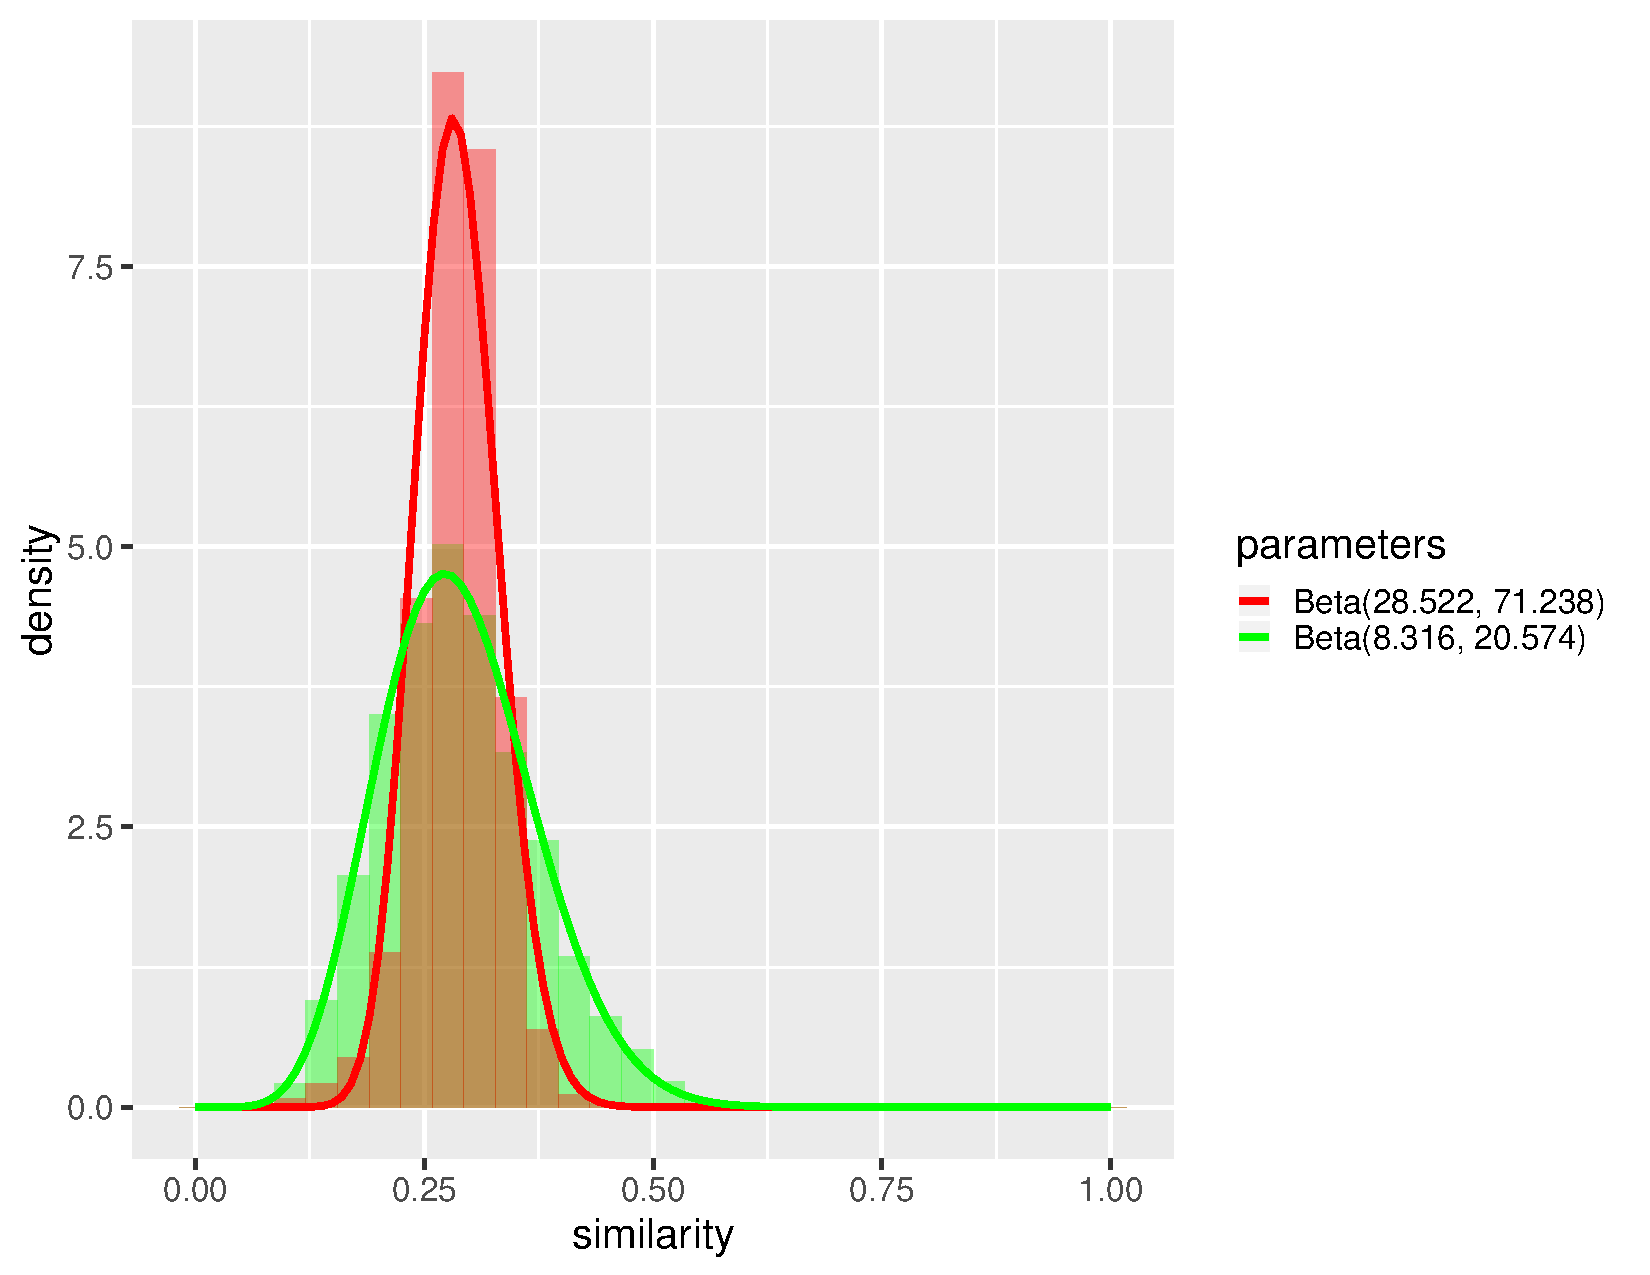
\includegraphics[width = .9\linewidth, height = .7\linewidth]{../../../Figures/paper_19_05/rh.pdf}
    \caption{Similarity between right helix elementary backscatterer and PolSAR data from the forest region (in green) and bare soil region (in red)}
    \label{fig:rh}
\end{figure}

\begin{figure}[!ht]
    \centering
    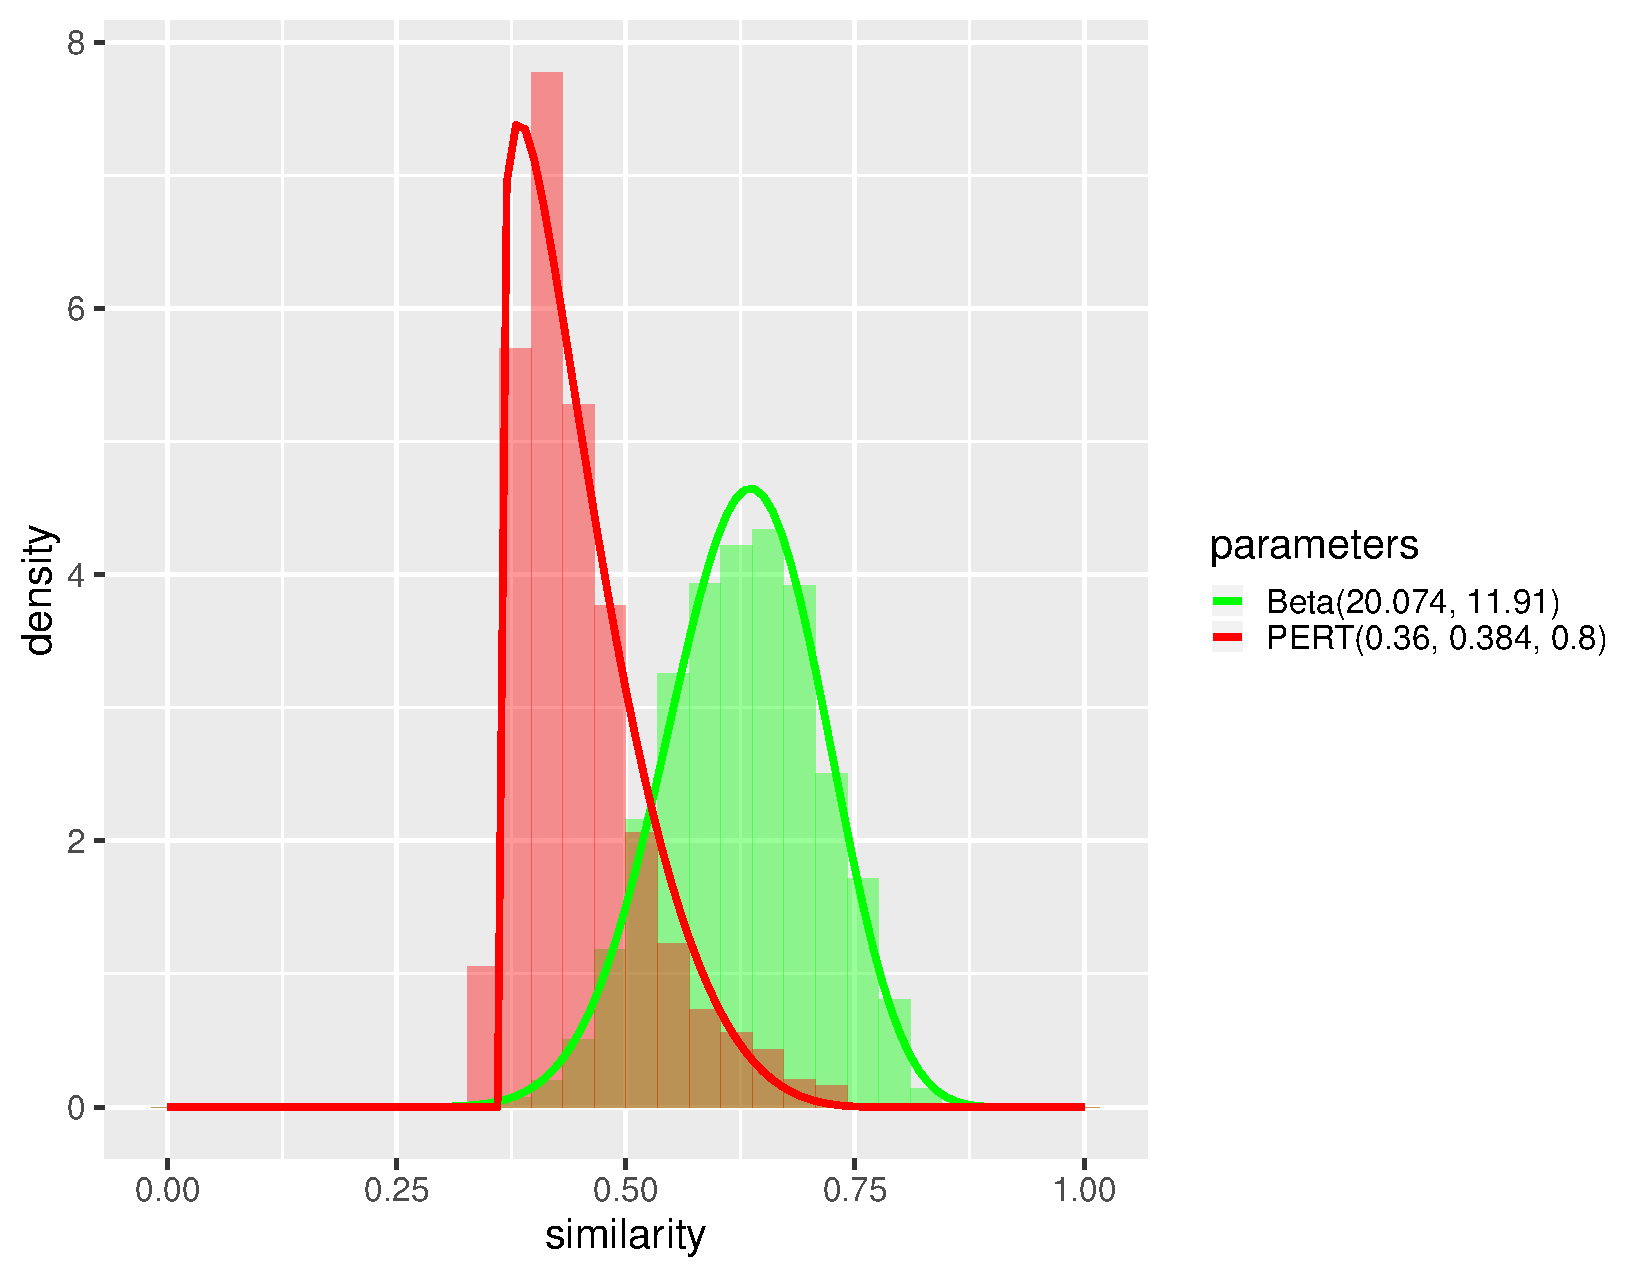
\includegraphics[width = .9\linewidth, height = .7\linewidth]{../../../Figures/paper_19_05/rv.pdf}
    \caption{Similarity between random volume elementary backscatterer and PolSAR data from the forest region (in green) and bare soil region (in red)}
    \label{fig:rv}
\end{figure}

\begin{figure}[!ht]
    \centering
    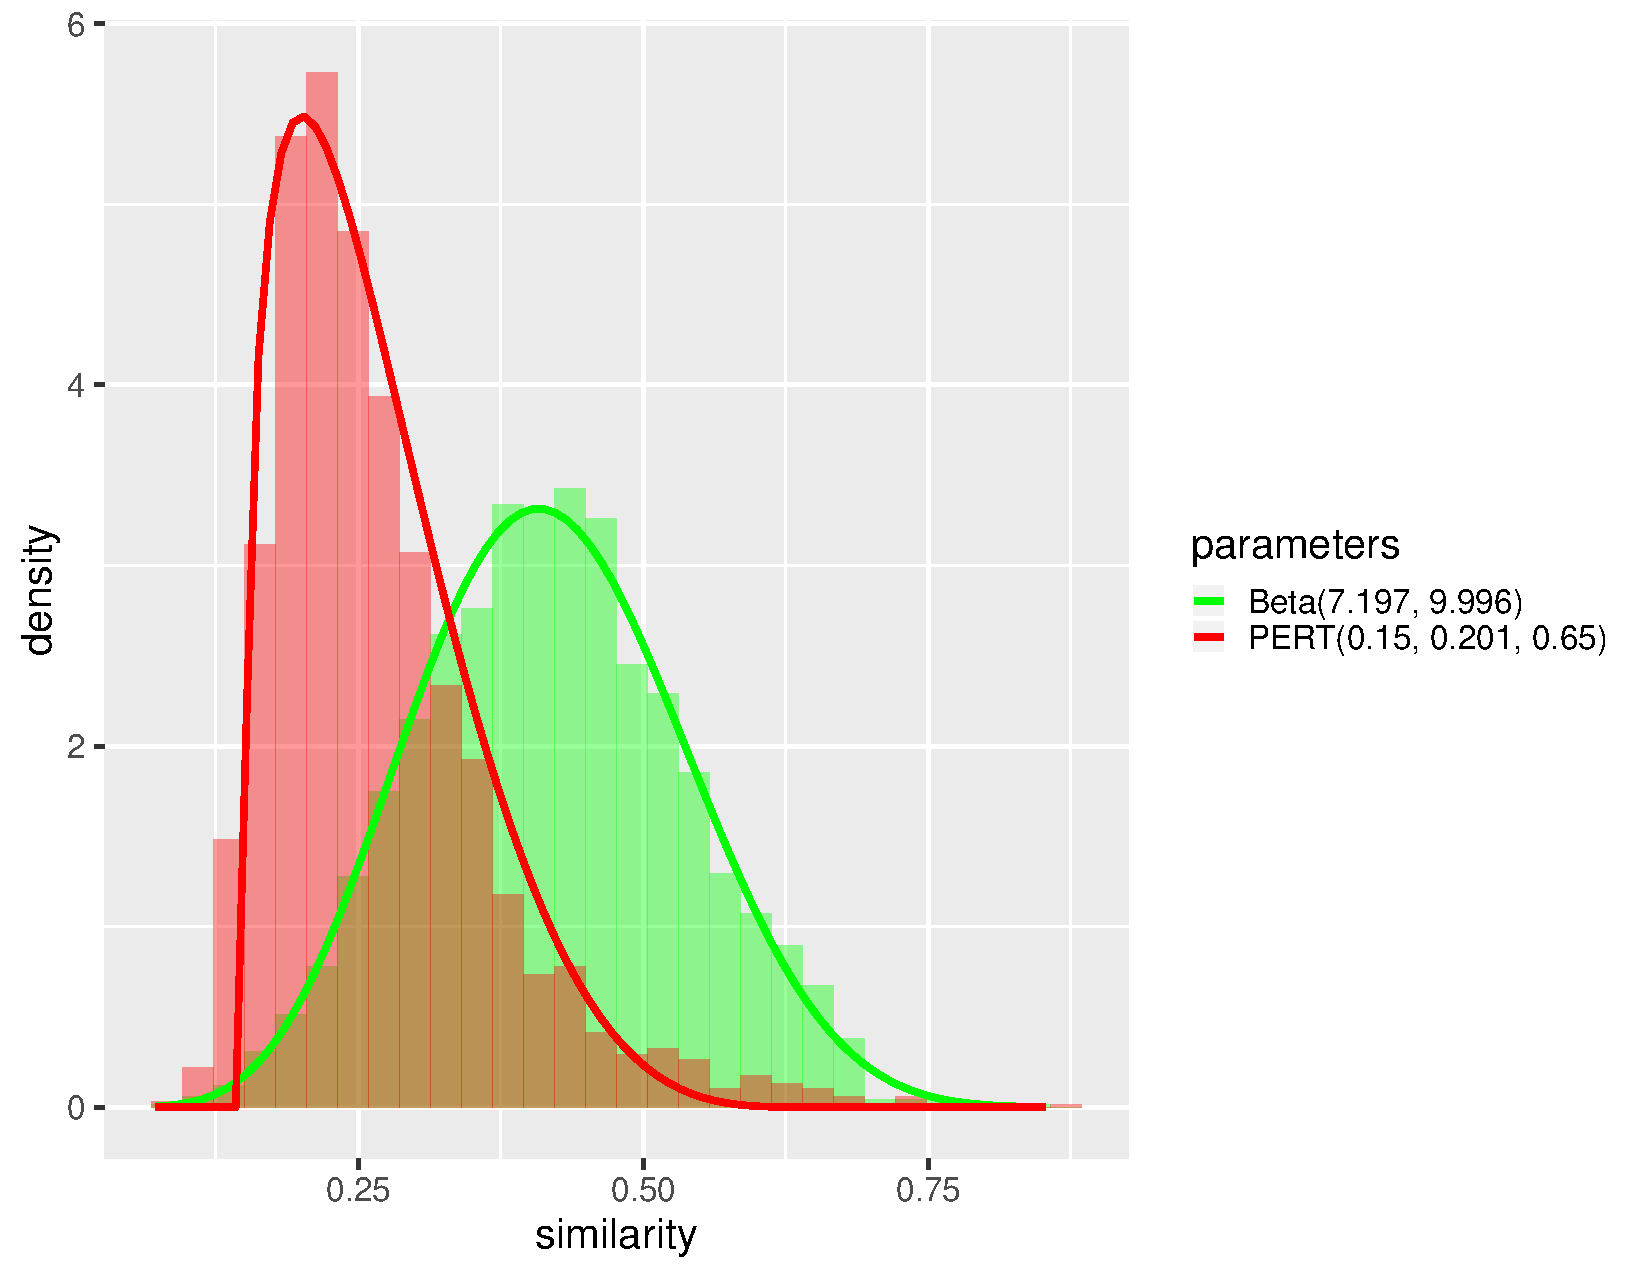
\includegraphics[width = .9\linewidth, height = .7\linewidth]{../../../Figures/paper_19_05/tr.pdf}
    \caption{Similarity between trihedral elementary backscatterer and PolSAR data from the forest region (in green) and bare soil region (in red)}
    \label{fig:tr}
\end{figure}

The table \ref{tab:estimated_params} contains the estimated parameters of the beta distribution to the analysied similarities. Through those, the probability density functions of the figures \ref{fig:wvn} to \ref{fig:tr} were adjusted to the histograms of the similarities. In addition, this table contains the estimate of the hope that results from the estimation of these parameters.

The probability density function of the beta distribution is given by

\begin{equation}
  f(x; a, c, \alpha, \beta) = \frac{(x - a)^{\alpha-1} (c - x)^{\beta - 1}}{B(\alpha, \beta) (c - a)^{\alpha + \beta - 1}}
\end{equation}

where B($\alpha$, $\beta$) is the beta function and a $<$ c.

In addition, the mean is given by

\begin{equation}
  \mu = \frac{\alpha}{\alpha + \beta}.
\end{equation}
\newpage
\begin{table}[!ht]
\centering
    \caption{Estimation of the hope and parameters of the beta distribution for similarities between the elementary backscatterers and the PolSAR data of the regions analyzed.}
    \label{tab:estimated_params}     
    \begin{small}
        \begin{tabular}{|*{6}{p{.12\linewidth}|}}
            \hline
             & \multicolumn{5}{c|}{$-1/4$-wave}\\
            \hline
             & $a$ & $c$ & $\alpha$ & $\beta$ & $\mu$\\
            \hline
            \textbf{Forest} & 0 & 1 & 7.83 & 22.758 & 0.255\\
            \hline
            \textbf{Bare soil} & 0.055 & 0.4 & 1.127 & 4.872 & 0.119\\
            \hline
        \end{tabular} 
    \end{small} 
    \vspace{.03\linewidth}
    \begin{small}
        \begin{tabular}{|*{6}{p{.12\linewidth}|}}
            \hline
             & \multicolumn{5}{c|}{$+1/4$-wave}\\
            \hline
             & $a$ & $c$ & $\alpha$ & $\beta$ & $\mu$\\
            \hline
            \textbf{Forest} & 0 & 1 & 8.681 & 23.277 & 0.271\\
            \hline
            \textbf{Bare soil} & 0.09 & 0.45 & 1.2 & 4.8 & 0.162\\
            \hline
        \end{tabular} 
    \end{small} 
    \vspace{.03\linewidth}
    \begin{small}
        \begin{tabular}{|*{6}{p{.12\linewidth}|}}
            \hline
             & \multicolumn{5}{c|}{Cylinder}\\
            \hline
             & $a$ & $c$ & $\alpha$ & $\beta$ & $\mu$\\
            \hline
            \textbf{Forest} & 0 & 1 & 7.5 & 12.165 & 0.381\\
            \hline
            \textbf{Bare soil} & 0.14 & 0.6 & 1.243 & 4.756 & 0.235\\
            \hline
        \end{tabular} 
    \end{small} 
    \vspace{.03\linewidth}
    \begin{small}
        \begin{tabular}{|*{6}{p{.12\linewidth}|}}
            \hline
             & \multicolumn{5}{c|}{Dihedral}\\
            \hline
             & $a$ & $c$ & $\alpha$ & $\beta$ & $\mu$\\
            \hline
            \textbf{Forest} & 0 & 1 & 5.38 & 36.87 & 0.127\\
            \hline
            \textbf{Bare soil} & 0.009 & 0.07 & 1.327 & 4.672 & 0.022\\
            \hline
        \end{tabular} 
    \end{small} 
    \vspace{.03\linewidth}
    \begin{small}
        \begin{tabular}{|*{6}{p{.12\linewidth}|}}
            \hline
             & \multicolumn{5}{c|}{Dipole}\\
            \hline
             & $a$ & $c$ & $\alpha$ & $\beta$ & $\mu$\\
            \hline
            \textbf{Forest} & 0 & 1 & 8.358 & 22.658 & 0.269\\
            \hline
            \textbf{Bare soil} & 0.075 & 0.35 & 1.625 & 4.374 & 0.149\\
            \hline
        \end{tabular} 
    \end{small} 
    \vspace{.03\linewidth}
    \begin{small}
        \begin{tabular}{|*{6}{p{.12\linewidth}|}}
            \hline
             & \multicolumn{5}{c|}{Narrow dihedral}\\
            \hline
             & $a$ & $c$ & $\alpha$ & $\beta$ & $\mu$\\
            \hline
            \textbf{Forest} & 0 & 1 & 5.89 & 33.198 & 0.15\\
            \hline
            \textbf{Bare soil} & 0.016 & 0.15 & 1.119 & 4.88 & 0.041\\
            \hline
        \end{tabular} 
    \end{small} 
    \vspace{.03\linewidth}
    \begin{small}
        \begin{tabular}{|*{6}{p{.12\linewidth}|}}
            \hline
             & \multicolumn{5}{c|}{Left helix}\\
            \hline
             & $a$ & $c$ & $\alpha$ & $\beta$ & $\mu$\\
            \hline
            \textbf{Forest} & 0 & 1 & 27.408 & 96.013 & 0.222\\
            \hline
            \textbf{Bare soil} & 0 & 1 & 8.38 & 24.286 & 0.256\\
            \hline
        \end{tabular} 
    \end{small} 
    \vspace{.03\linewidth}
    \begin{small}
        \begin{tabular}{|*{6}{p{.12\linewidth}|}}
            \hline
             & \multicolumn{5}{c|}{Right helix}\\
            \hline
             & $a$ & $c$ & $\alpha$ & $\beta$ & $\mu$\\
            \hline
            \textbf{Forest} & 0 & 1 & 28.522 & 71.238 & 0.285\\
            \hline
            \textbf{Bare soil} & 0 & 1 & 8.316 & 20.574 & 0.287\\
            \hline
        \end{tabular} 
    \end{small} 
    \vspace{.03\linewidth}
    \begin{small}
        \begin{tabular}{|*{6}{p{.12\linewidth}|}}
            \hline
             & \multicolumn{5}{c|}{Random volume}\\
            \hline
             & $a$ & $c$ & $\alpha$ & $\beta$ & $\mu$\\
            \hline
            \textbf{Forest} & 0 & 1 & 20.074 & 11.91 & 0.627\\
            \hline
            \textbf{Bare soil} & 0.36 & 0.8 & 1.218 & 4.781 & 0.449\\
            \hline
        \end{tabular} 
    \end{small} 
    \vspace{.03\linewidth}
    \begin{small}
        \begin{tabular}{|*{6}{p{.12\linewidth}|}}
            \hline
             & \multicolumn{5}{c|}{Trihedral}\\
            \hline
             & $a$ & $c$ & $\alpha$ & $\beta$ & $\mu$\\
            \hline
            \textbf{Forest} & 0 & 1 & 7.197 & 9.996 & 0.418\\
            \hline
            \textbf{Bare soil} & 0.15 & 0.65 & 1.408 & 4.592 & 0.267\\
            \hline
        \end{tabular} 
    \end{small} 
\end{table}

\section{Goodness-of-fit test}

For the Kolmogorov-Smirnov goodness-of-fit test, it was selected 400 samples from the forest region and 120 samples from the bare soil region through simple random sampling method and realize the test for all elementary backscatterers with respect the respective distributions in the figures \ref{fig:wvn} to \ref{fig:tr}. The table \ref{tab:pvalues_table} contains the p-values obtained by the tests, which the least p-value is 0.07. 

\begin{table}[!ht]
\centering

    \caption{P-values obtained by Kolmogorov-Smirnov goodness-of-fit test for all elementary backscatterers}
    \label{tab:pvalues_table}     

    \begin{small}
    
        \begin{tabular}{|*{6}{p{.12\linewidth}|}}
            \hline
             & $-1/4$-wave & $+1/4$-wave & Cylinder & Dihedral & Dipole\\
            \hline
            \textbf{Forest} & 0.979 & 0.808 & 0.763 & 0.733 & 0.975\\
            \hline
            \textbf{Bare soil} & 0.361 & 0.893 & 0.264 & 0.443 & 0.475\\
            \hline
        \end{tabular} 
    \end{small} 
    \vspace{.05\linewidth}
    \begin{small}
    
        \begin{tabular}{|*{6}{p{.12\linewidth}|}}
            \hline
             & Left & Narrow & Random & Right & Trihedral\\
             & helix & dihedral & volume & helix & \\
            \hline
            \textbf{Forest} & 0.959 & 0.787 & 0.589 & 0.344 & 0.582\\
            \hline
            \textbf{Bare soil} & 0.099 & 0.206 & 0.480 & 0.072 & 0.127\\
            \hline
        \end{tabular} 
    \end{small} 
\end{table}

\bibliographystyle{IEEEtran}
\bibliography{../../../Bibliography/references}

\end{document}

